%Quinto ejercicio.
\documentclass{standalone}
\usepackage[utf8x]{inputenc}
\usepackage[T1]{fontenc}
\usepackage{PTSansNarrow}
\usepackage[usenames,dvipsnames,x11names,table,svgnames]{xcolor}
\usepackage{tikz}
\usetikzlibrary{babel,calc}
\begin{document}

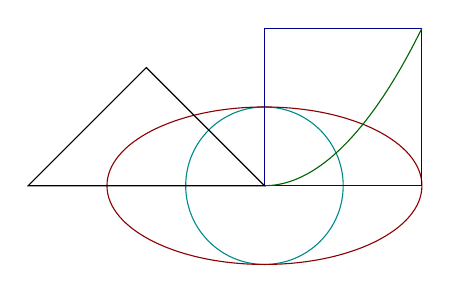
\begin{tikzpicture}
\draw[DarkCyan](0,0) circle[radius =1];
\draw[DarkRed] (0,0) ellipse[x radius =2, y radius =1];
\draw[DarkBlue] (0,0) rectangle (2,2);
\draw[DarkGreen](0,0) parabola (2,2);
\draw (0,0) -- (-3,0) -- (-1.5, 1.5) -- cycle;
\end{tikzpicture}

\end{document}